%! Suppress = MissingImport
\section{Waterfall Methodology}\label{sec:waterfall-methodology}
%https://en.wikipedia.org/wiki/Waterfall_model#History
The waterfall methodology was first introduced in the 1950's by Mr.
Benington but was only formalized in 1970 by  Winston W. Royce.
This methodology has been widely used in the industry, although it received
a lot of criticism few decades after.

This section will first present the key concepts of this methodology followed
by the detailed workflow.
After that, we'll point out its weaknesses and present a improved version:
the V-model.
Finally, we'll state the residual problems and limits of the improved model.

\subsection{Key concepts}\label{subsec:key-concepts}

The two main phases in software development are \textit{Analysis} and
\textit{Coding}.
Even projects with no clear methodology will at least go throw those two phases
that define and build the software.
However, these steps are only the emerged part of the iceberg.
Any software will require some specific design regarding its architecture, the
technologies it will use, its production environment and will also need time
to verify that the software actually works.

\begin{figure}
    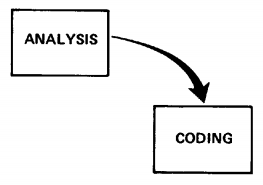
\includegraphics{../../images/waterfall/figure_1}
    \centering
\end{figure}

The problem stated by Royce is that these design and testing steps were not very
well regarded, simply because they didn't directly add any business value.
Therefore, these steps were not very valuable from a client point of view and
were likely to be skipped. \\
Ignoring these steps often leads to horrific and costly overrun.
For example, fixing an architectural issue in a software might require a
complete new design and the developers will have to start all over again.
Also a lot of bugs will only be uncovered in production because of a lack
of testing effort, in terms of both strategy and execution.
New versions of the software will have to be made in order to fix them, while
hoping not adding new problems.

Royce then proposed a model that adds extra steps to the development process,
to better design the software before implementing and better test it before
releasing it.

We'll see more details later about the workflow itself.
The main improvement is that we now have more design steps, a dedicated step
for testing and also one for the operations phase.
These steps that aren't directly related to the business value of the
software are now part of the nominal development process.

%TODO remove this figure as we do not describe the steps in the workflow ?
\begin{figure}
    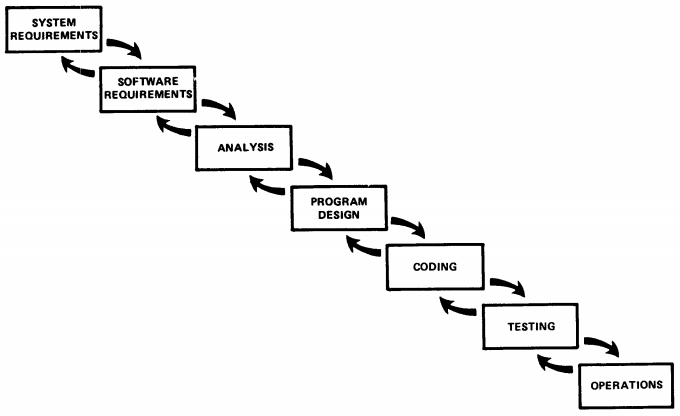
\includegraphics[scale=0.9]{../../images/waterfall/figure_2}
    \centering
\end{figure}

\subsubsection{Documentation}

This emphasis on the design of the software makes the waterfall very
document-oriented.
This is one of the main traits of this methodology and there're a several
types of documents:
Software requirements, preliminary program design, interface design, final
program design, test plan and operations instructions.
These documents will help in several ways the project.

The formal aspect of written documents are nice during the design
specification by providing a tangible evidence of the understanding of a
requirement or the definition of a program interface.
A misunderstanding can easily be detected during a read over phase, by the
author, the analysts and the client.
This also prevent the project from forgetting a feature or any detail mentioned
during an informal meeting.

The documentation externalizes the knowledge from the analysts and clients
minds, which will benefit the whole project team.
Future maintainers of the application won't have to dig into the code base to
understand what it does, they will simply have to look at the structured
documentation to do so.

The operations phase will also take advantage of a well documented
application.
Installation or deployment processes will be clearly defined and even people
that  weren't there during the development phase will be able to start and
run the program.

\subsubsection{Testing}

The waterfall methodology also puts testing a bit more at upfront, by adding
it as a required step in the development process.

As we mentioned it in the previous section, this methodology is very
document-oriented and this becomes very handy for the testing phase.
The documentation provides a comprehensive overview of all the requirements
and features of the application, this will greatly help for the test
strategy.

The strategy will drive the design of test cases and also define the
required data set to execute them.
This test plan is very important and is made even before the implementation
phase, to ensure that the validation of the final product is doable.

Once the strategy is done, the test cases redaction can be started at any
time, whether before, after or in parallel of the implementation phase.
This let the time to the test team to nicely prepare the test phase.

% TODO remove this bulky figure ? Will the associated section still be ok ?
\begin{figure}
    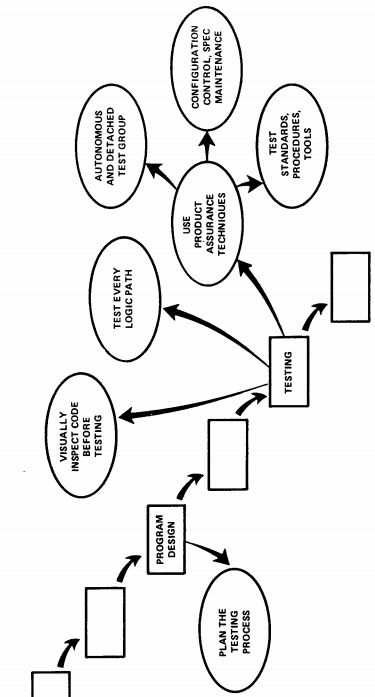
\includegraphics{../../images/waterfall/figure_3}
    \centering
\end{figure}

\textit{Documentation} and \textit{Testing} are really the two new main
concepts of the waterfall methodology.
The documentation helps to structure the software development process and
makes easier to write and execute.

\subsection{Workflow}\label{subsec:workflow}

This section is going to describe the workflow of the waterfall methodology.
Going from the design phases to the operations, it'll cover how the
different teams work in each phase.
Some steps have been grouped into to a single sub section to make the
workflow smoother.

%https://www.guru99.com/hp-alm-introduction.html
The workflow will be illustrated with the use of an Application
Lifecycle Management tool.
An ALM tool is here too help the end-to-end management of a software project,
from the design to delivery.
All the requirements, specifications, test plans etc.
are centralized in this kind of tool.

\begin{figure}
    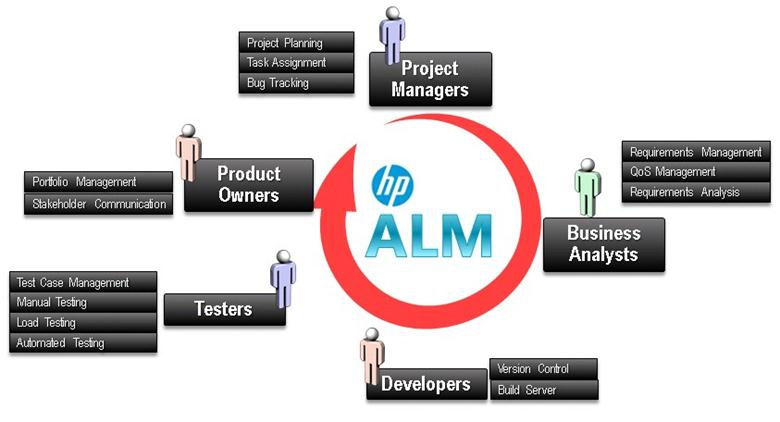
\includegraphics{../../images/waterfall/alm_workflow.jpg}
    % TODO fix alignement
\end{figure}

\subsubsection{Design phase}
The design phase is the first and most important in waterfall.
This phase can be decomposed into several steps: gather the customer
needs, define the requirements and design the solution.
Let's dig into each step.

The gathering of the customer needs is the first step of the design phase.
This is where the client presents its high level business needs to the
analysts and architects.
This can be done through workshops, meetings, presentations etc.
The commonly used supports are word documents or slides.

Once the analysts and architects have a clear understanding of the customer
needs, they will propose an architecture and the requirements.
Even if the solution isn't fully defined yet, the global architecture should be
able to fulfil all the requirements.

The requirements can be seen as a low-level representation of the customer
needs.
They are written by the analysts, validated by the client and managed using
the ALM tool, in order to keep them organized, centralized and formalized.

When the proposed architecture and requirements are validated by the client,
the specification of the solution can start.
In this phase, each requirement is analyzed and declined into a sub set of
specifications that will satisfy it.
These specifications can be either functional or non-functional.
The difference between the two is that a functional specification will
describe how the system should \textit{behave}, where the non functional will
define \textit{how} to do it.

All specifications will also be stored in the ALM tool and be mapped to
the requirements they cover.
One great advantage of an ALM tool is to compute the coverage of the
specifications.
We can see at a glance if there is a requirement that is not associated to at
least one specification.
This will prevent us from forgetting a requirement during the specification
phase.

\subsubsection{Test Strategy}
This step can be done by the analysts that wrote the specification or could be
handled by a complete external team, made of dedicated professional testers.
Thanks to all the documentation written in the design phases and the ALM tool,
it's indeed possible to externalize the testing phases and the project will be
able to leverage the experience of these professional testers.

During the test strategy, every specification is analyzed to determine which
acceptance test suite must be run in order to validate the feature.
The global workflow, dataset, environment setup etc.
Everything is planed before to make sure that the actual software design and
architecture can be validated in the end.

The ALM tool is again very useful because it allows to compute the coverage
of our specifications.
It's the same principle as the previous section, it simply checks if every
requirement as at least one associated test.
The coverage however can sometime be misleading because it may be complex to
represent every possible path for every requirement.
Therefore a requirement can be covered by a test, but in fact there's only one
nominal test case, and the other rare, but possible, patsh are not tested.

\subsubsection{Implementation}
% TODO read over
% TODO add a basic dev workflow
Once the implementation phase completed, some
preliminary checks must be done by the developers, like visual inspection
by a peer or code reviews.
A certain amount of bugs can therefore be immediately fixed at a very low cost.
After these checks are done, the real testing phase can start.

\subsubsection{Testing phase}
% TODO read over
% TODO add the use of test / ALM tools
All the test cases written following the testing strategy are executed by the
testers.
Every bug or unexpected behaviour will raise a new defect.
The defect are collected at the end of testing phase and given to the dev
team to fix them.

The previously failed tests are then executed again to ensure that the bug
are fixed.
This cycle is repeated until there is no more defects, then only the testing
phase can end.

\subsection{Limits}\label{subsec:limits}

\subsection{V-Model}\label{subsec:v-model}